\section{Future Work}
\label{sec:future}

\subsection{Trusted Function Runtime}

For the purposes of the \SystemName libaray and \SystemName-Lite system, we've claimed that the proxy/cloud provider can be untrusted.
This isn't exactly true in the system as we've presented it, since the instances still rely on the proxy to obtain key material (public parameters) to create their keys, and the keys are in the memory of these instances which are running on the cloud provider's hardware.
In order to make this threat model assumption hold, the eventual Knative \SystemName extension, will have to run its function instances in Trusted Execution Environments (TEEs) on hardware capable of doing so.
%
For \SystemName's function runtime, we will extend \emph{Project Oak},\footnote{
\url{https://github.com/project-oak/oak}
%\url{https://nordprojects.co/projects/oak/}
}
an open-source framework for processing private data within a TEE\@.
%
The central component of Project Oak is the \emph{Oak Functions} platform (see
Figure~\ref{fig:oak}), which executes each function in a confidential VM with a
custom, minimal operating system kernel designed to execute only a single
process.
%
\begin{figure}
    \centering
    \includegraphics[page = 3, width=0.48\textwidth]{diagrams/slides.pdf}
    %
    \caption{Oak and DICE architecture.
    %
    In the DICE model, each software layer loads and measures the next layer,
    generates an ephemeral key pair for the layer, and issues the layer a
    certificate endorsing its measurement and public key.
    %
    Oak uses AMD's trusted hardware as the root of trust.
    %
    % In total, Oak's implementation of DICE results in a certificate chain, rooted
    %in the AMD trusted hardware, that attests the entire workload.
    }
    \label{fig:oak}
\end{figure}
%
The function runs in a secure WebAssembly (Wasm) runtime sandbox, preventing
the process from leaking any sensitive client data.
%
Additionally, Oak uses the DICE~\cite{24-misc-dice} architecture for measured
boot to extend AMD SEV-SNP's attestation from the initial state of the VM
to the entire VM workload.
%
We will modify the Oak kernel with cryptographic support to transparently
manage keys and encrypt I/O\@.


\subsection{Control Flow Integrity}
%
Beyond encrypting function I/O, \SystemName must ensure the integrity
of the sequence of functions.
%
%Guaranteeing this property is challenging, as a function chain can span multiple
%organizations, and an organization may be unaware of its functions position in
%the chain.
%
\SystemName approaches this challenge in two ways.
%
First, we extend the Oak runtime to include a cryptographically binding record
of provenance: each function extends a path signature by signing over its
current link.
%
The last function then posts this provenance record to an untrusted log that
any organization can monitor and audit.
%
Additionally, if an organization knows a flow graph for the function chain (or
some subset thereof),  Oak will locally verify that the received event and the
function's subsequent output conform to the graph.


\subsection{Optimization}
%
\SystemName relies on certificate chains both for attestation and provenance.
%
To reduce bandwidth and storage costs, \SystemName can compress the chains
using an aggregate signature
scheme~\cite{03-eurocrypt-aggregate_signatures_bilinear_maps}.
%
In an \emph{aggregate signature},
each private key $sk_i$ signs a \emph{distinct} message $m_i$ to form signature
$\sigma_i$, and any party can compress the $\sigma_i$ into a single,
small aggregate signature $\sigma^*$.  
%
The aggregate signature convinces a verifier that each signer signed their
respective message.

%% \textbf{adwait "discussion"}
%% % Discussion (discuss some of the important simplifying assumptions, and
%% % suggest possibilities for future work)
%% 
%% Notably, to get any benefit from SAMBA, users will have to use one of the three open source FaaS orchestrators (whichever we decide on), and run only Oak Restricted Kernel VMs.
%% It's doubtful that this will become the standard for FaaS workloads, since most in-use FaaS systems, such as AWS Lambda, use proprietary software.
%% SAMBA's practical in-market use cases are therefore likely next to none, but it serves as a good proof of concept for how to add these security features to FaaS systems.
%% 
%% As noted in the threat model, side channel attacks are out of scope for this project.
%% This assumption simplifies things greatly, since side-channel attacks are definitely feasible in the modern cloud. \cite{zhao_everywhere_2024} \cite{zhao_last-level_2024}
%% I acknowledge that it's a bit fantastical to assume that the cloud provider could be malicious, but woudlnt' think to perform a side-channel attack on our otherwise largely protected system.
%% Defenses against side-channel attacks in the cloud are another active research area.
%% It is unfortunate that strengthening overall security and hardeing against side-channel attacks seem to both leave the other vulnerable.
%% Uniting solutions for these two issues without significant performance impact is an interesting research area worthy of pursuit.
